\chapter{Introduction}\label{ch:introduction}


\section{Background}Statistical graph or plot of data has its presence way before the development of the classical inference procedures. The first recorded instance of statistical graphics based on the data was known to be in the year 1644 (variations in determination of longitude between Toledo and Rome as illustrated by \cite{friendly:2001}). The development of fundamental classical inferential procedures took around two hundred years from Bernoulli through Fisher (1713 to 1935 as per \cite{hald:2004}). 

The power of statistical plots in statistical data analysis is widely acknowledged. Model diagnostics or exploratory data analysis is predominantly dependent on statistical plots and visualization through human observation. \cite{cleveland:1984} talks about the visual perception and the development of graphical methods. Statistical graphs has been widely used for going beyond the standard paradigms of estimation and testing, to look for patterns in data beyond the expected. As pointed out in Gelman [2004], improvements in computation has helped in the developments of statistical graphics. Higher resolution graphics, more sophisticated user interfaces and accessible software had made graphical methods to be more widely available. A grammar of graphics introduced by \cite{wilkinson:1999} presents a structured way to generate specific graphics from data and define connections between disparate types of plot. The problem is though we can represent our findings using statistical graphics, there is possibly no way to say what we see is real. 

% to look presentation of findings. The question is whether we can use this powerful tool, the statistical plots, to make statistical inference. This has been a open question until recently when \citet{buja:2009} presented formal structure of the visual inference procedure to detect the significant pattern in the data.

%
%I intend to write down a little history of the statistical graphics in this section. The goal is to identify why the graphics were not used as a tool for statistical inference even though we see its presence way before the development of classical inference techniques. One factor could be the absence of modern computing facilities. But to what extent does the lack of computing facility prevent statistical graphics from being used as the tool for statistical inference?

%\newpage

\section{Review of Hypothesis Testing}

Classical statistical inference can be broadly classified into two categories, namely Estimation and Testing of hypothesis. In testing of hypothesis we start out with a claim or belief about the population parameter. We need to verify the claim or belief based on whether our sample data matches the belief. In any test, there are two competing hypothesis. The null hypothesis denoted by $H_0$ is a statement of what we assume to be true which reflects the current condition about the population parameter. On the other hand, the alternative hypothesis, denoted by $H_a$ which is a statement against the null hypothesis $H_0$ is what we want to show. 

The philosophy behind a statistical hypothesis is the same as in a jury trial. There are only two possibilities:
\begin{itemize}
\item ``not guilty'' corresponding to $H_0$
\item ``guilty'' corresponding to $H_a$ 
\end{itemize}
Like in a jury trial the philosophy is ``innocent until proven guilty'', we assume $H_0$ is true until we have sufficient evidence in the data in favor of $H_a$. 
We may have three different types of alternative hypotheses against the null hypothesis. Let us assume we want to test for a population mean $\mu$. So against the null hypothesis $H_0: \mu = \mu_0$, we may have
\begin{itemize}
\item $H_a: \mu > \mu_0$
\item $H_a: \mu < \mu_0$ 
\item $H_a: \mu \ne \mu_0$
\end{itemize}
where $\mu_0$ is some pre-specified value that we assume holds true under $H_0$. The first two alternative hypotheses is known as one-sided alternatives and the third one is known as two-sided alternative. Also $H_0$ and $H_a$ should always contradict each other.

Let us assume that we want to test $$H_0: \mu = \mu_0 \qquad \hbox{vs} \qquad H_a: \mu > \mu_0$$
Now based on the sample we have in hand, we calculate the appropriate sample statistic. So in this case we calculate the sample mean $\bar{X}$ and $S$. If $H_a$ is indeed true, we should expect $\bar{X}$ to be greater than $\mu_0$. Then the question of interest is how much greater than $\mu_0$ should $\bar{X}$ be before we start doubting the null hypothesis. In other words, is a value of $\bar{X}$ unusually large if $H_0: \mu = \mu_0$ is supposed to be true. If the answer is yes, then that would be evidence against $H_0$ in favor of $H_a$. To assess how unusual or unlikely our data is and hence the corresponding sample mean, we may look where the estimate of the standardized score falls on the distribution under $H_0$.  For more details take a look at \cite{kutner:2005}.

Assuming that the sample comes from a Normal population or the sample size is large enough so that the sampling distribution of $\bar{X}$ is approximately Normal, the standardized score or the test statistic under $H_0$, also known as, $t$-score is given by
$$t = \frac{\bar{X} - \mu_0}{S/\sqrt{n}}$$
Under $H_0$, $t$ follows a $t$ distribution with $n - 1$ degrees of freedom.

In general we can write a test statistic for any population parameter as 
$$\frac{\hbox{sample estimate of parameter} - \hbox{hypothesized parameter value under }H_0 }{\hbox{standard error of the estimator}}$$ 
Under different situations, the test statistic follows different distributions. If the observed value of the test statistic is extreme, we would have reasons to believe that the data comes from a population with population mean $\mu > \mu_0$. Automatically, the question arises how extreme can the test statistic be when we start believing the data comes from a population with population mean greater than $\mu_0$. 

 Here we define something that is typically known as Type I error or the level of significance. The level of significance, denoted by $\alpha$ corresponds to the error rate that we allow ourselves saying that in 100$\alpha$ \% of all decisions we will make the wrong decision, i.e. we will reject the null hypothesis $H_0$ when in fact $H_0$ is true. 
 
 Hence we look at the value of 100(1 - $\alpha$) percentile of t distribution with the appropriate degrees of freedom and if the observed value is greater than the value, we reject $H_0$, otherwise we fail to reject $H_a$. So
 \begin{itemize}
 \item Reject $H_0$ if $t_{\hbox{obs}} > t_{1 - \alpha}$
 \item Fail to reject $H_0$ if $t_{\hbox{obs}} < t_{1 - \alpha}$
 \end{itemize}
Similarly for a two sided alternative, we have 
  \begin{itemize}
 \item Reject $H_0$ if $|t_{\hbox{obs}}| > t_{1 - \alpha/2}$
 \item Fail to reject $H_0$ if $|t_{\hbox{obs}}| < t_{1 - \alpha/2}$
 \end{itemize}
 We may also make the decision based on so-called p-value. As defined in \cite{moore:2009}, the p-value is defined as the probability of getting a value at least as unusual as the observed sample statistic assuming that $H_0$ is true. Hence the p-value measures evidence against $H_0$. The smaller the p-value the stronger the evidence is against the null hypothesis $H_0$ and in favor of $H_a$. As previously discussed, the p-value is compared to the level of significance $\alpha$ to make the decisions.
  \begin{itemize}
 \item Reject $H_0$ if p-value $<$ $\alpha$
 \item Fail to reject $H_0$ if p-value $>$ $\alpha$
 \end{itemize}
 Type I error or the level of significance, denoted by $\alpha$, is the probability of rejecting the null hypothesis $H_0$ when $H_0$ is true. Type II error, denoted by $\beta$ is the probability of failing to reject the null hypothesis $H_0$ when $H_0$ is false. Type I error is committed in a jury trial when there is ``no guilty'', a person is convicted as ``guilty''. This is a serious mistake as an innocent person is convicted. Type II error is committed when there is a ``guilty'' but he was not convicted. The power of a statistical test is defined as the probability of rejecting the null hypothesis $H_0$ when $H_0$ is false and is denoted by 1 $-$ $\beta$. \\
 
More generally, let $\theta$ be a population parameter of interest, with $\theta$ $\in$ $\Theta$, the parameter space. Any null hypothesis $H_0$ then partitions the parameter space into $\Theta_0$ and $\Theta_0^c$ with $H_0: \theta \in \Theta_0$ versus $H_a: \theta  \in \Theta_0^c$ as defined in \cite{casella:2002}. \\

Let $\chi$ be the set of all possible values of $\mathbf{X} = (X_1, \dots, X_n)$. Then a test function or a test rule $\phi(X_1, \dots, X_n)$ is a function from $\chi$ into [0, 1] with the interpretation that if $\mathbf{X} = (X_1, \dots, X_n)$ is observed then $H_0$ is rejected with probability $\phi( \mathbf{X})$. Hence the following definitions:
\begin{itemize}
\item Probability of Type I error at $\theta \in \Theta_0$ is $E_{\theta} \phi(\mathbf{X})$. 
\item Probability of Type II error at $\theta \in \Theta_0^c$ is $1 - E_{\theta} \phi(\mathbf{X})$. \item Size or the level of the test function $\phi(\mathbf{X})$ is given by $\max_{\theta \in \Theta_0} E_{\theta} \phi(\mathbf{X}) $.
\item Power function of $ \phi(\mathbf{X})$ is given by $\Pi_{\phi}(\theta) = E_{\theta} \phi(\mathbf{X})$.
\end{itemize}


\section{Introduction to Visual Inference} \citet{buja:2009} proposes visual statistical methods with an inferential framework. In visual inference the plots take on the role of test statistics, the test statistic is not a real number anymore. Assuming that the null hypothesis is true, several other plots are generated. These plots, known as the null plots gives the ``null distribution of plots'' analogous to the null distribution of test statistics. Though the null distribution is infinite i.e. conceptually we may have an infinite collection of plots of `null datasets', in practice we sample a finite number of null datasets and generate a gallery of null plots. The observed plot, which is the test statistic, is presented along with the null plots to several viewers. If the observed plot show a specific pattern not seen in the null plots, we will have reasons to believe that the observed plot may not have come from the null distribution. Hence if the viewer correctly identifies the observed plot , the decision is to reject the null hypothesis. To formalize the process of visual discovery the paper proposes two protocols described in the next section. As they said in their paper, each of the protocols helps to quantify the strength of signal versus noise similar to numerical hypothesis testing. 

\subsection{Protocols of Visual Inference} \label{sec:protocol} \citet{buja:2009} introduces two protocols for graphical inference: one is the  ``Rorschach'' and the other is the ``lineup''. The purpose of the Rorschach protocol is to measure a data analyst's tendency to over interpret plots in which there is no or spurious structure. On the other hand the lineup provides a simple inferential process to produce a valid p-value for the observed plot. Here we describe the protocols briefly and refer the reader to \citet{buja:2009} and \cite{hadley:2010} for more details. \\

{\bf Rorschach:} It is possible that the randomness of the data inherits some pattern in the plot. The Rorschach protocol is designed to expose the data analyst's tendency of over-interpretation of patterns when there is actually no or spurious structure. The results are specific to a particular data analyst and a particular data analysis procedure. The protocol estimates the effective family-wise Type I error rate. A data administrator may generate the null plots and decides about the prior information that the data analyst is provided. The administrator may program the series of null plots in such a way that the plot of the real data is inserted in a random location. A toned-down version may also be used for self training. This self training may improve the family-wise error rate of the data analyst and develop an awareness of the features they are most likely to spuriously detect. 
%The human eye can see pattern while there is no pattern in deed. This protocol helps understand the extent of this pattern in the null plots. The process includes asking readers to report what they see in null plots. This helps reader getting acquainted with the natural patterns due to completely randomness. 
The Rorschach protocol is named after the (pop-)psychology Rorschach test, in which subjects interpret abstract ink blots. \\

{\bf Lineup:} The lineup protocol gets its name after the police lineup of criminal investigation. In a police lineup, the accused is placed among a set of innocent people who may be prisoners, actors or volunteers having no connection with the case. The witness is asked to pick from this lineup. Likewise in a lineup protocol, the accused which is the observed plot is placed randomly among a set of null plots, say $m$, and the witness (in this case the viewer) is asked to identify the plot as most different from the others. If the viewer  can correctly identify the observed plot from the lineup, we have reasons to believe that the observed plot has a specific pattern which is missing in the null plots. This protocol leads to the development of the technique of visual inference by defining the test statistic as a plot that mostly show a specific pattern in the data when alternative hypothesis is true. Figure \ref{lineup} shows a typical lineup. \\

Let us consider the following example . The data represents the concentration of a metal in mg/kg for two sites A and B.
%Model : $Y_i$ = $\beta_0$ + $\beta_1 X_i$ + $\epsilon_i$, \qquad $\epsilon_i \stackrel{iid}{\sim} N(0, \sigma^2)$ \\
%\vspace{0.1cm}
We want to test whether there exists a significant difference between the concentration levels in the two sites A and B. Let $\mu_1$ denote the mean concentration level in Site A and $\mu_2$ denote the mean concentration level in Site B. To test that, we have the following null and alternative hypothesis:
\[
H_0: \mu_1 = \mu_2 \qquad \hbox{versus} \qquad H_a: \mu_1 \ne \mu_2
\]
%\vspace{0.4cm}
The test statistic is the plot of the real data. The 19 null plots are generated by assuming that null hypothesis $H_0: \mu_1 =  \mu_2$ is true. So we permute the class variable site to obtain the null plots keeping the other variables fixed. The observed plot is placed randomly among these 19 plots in a lineup given in Figure \ref{lineup}. The viewer is asked to identify the plot which is most different. If the viewer can identify the plot of the real data, we will have reasons to believe that the observed plot has a pattern which is absent in the null plots. So we would reject the null hypothesis. If the viewer cannot identify the observed plot, we fail to reject the null hypothesis. \\
%\newpage

\begin{figure}[hbtp]
%\begin{figurehere}
   \centering
       \scalebox{1}{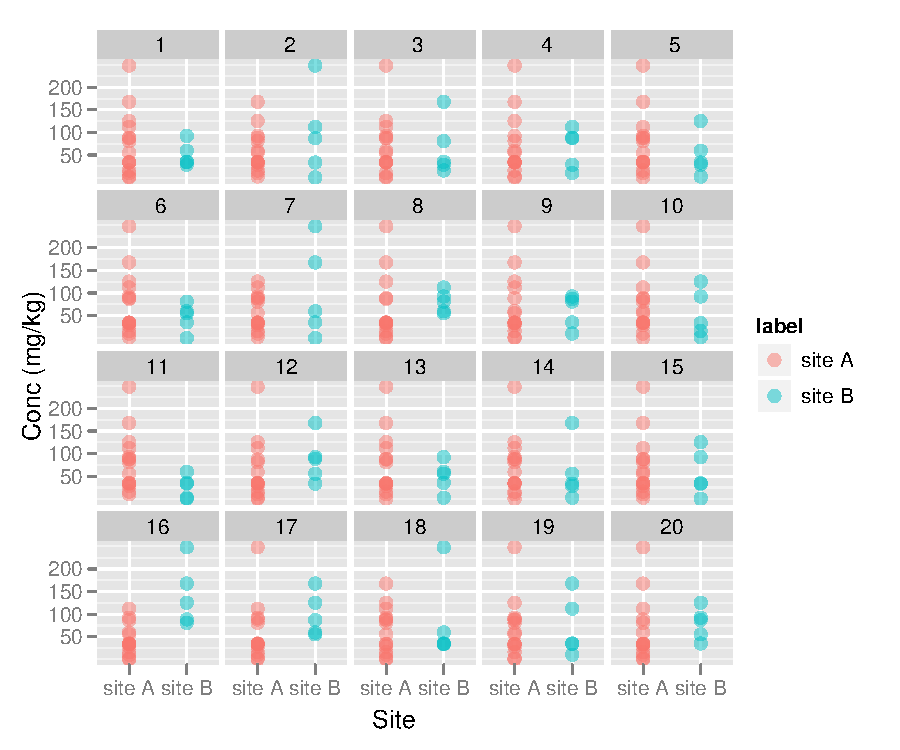
\includegraphics{lineup-dot.pdf}}
      \caption{A typical lineup plot ($m = 20$) for testing $H_0: \mu_1 =  \mu_2$. 
      % \qquad vs \qquad H_a: \beta_1 \ne 0$
      When the alternative hypothesis is true the observed plot should have the largest vertical difference between the centers. Can you identify the observed plot?}
      \label{lineup}
%	\vspace{-.1in}
\end{figure}

Plot 16 is the plot of the real data. If the viewer could identify the plot then we have reasons to believe that there exists a statistically significant difference between the mean concentration levels in site A and site B. So the lineup protocol is the basis of the visual inference while the Rorschach protocol helps viewer understand the extent of randomness. \\

Later in 2010, \cite{majumder:2010} did a comparative study between the visual inference method and the classical inference methods by comparing the expected power of the visual test and the power of the UMP test. They showed that the expected power of a visual test is almost as good as the power of UMP test. They established properties and efficacy of visual testing procedures in order to use them in situations where traditional test cannot be used. \cite{majumder:2010} in their paper have this stunning table (Table \ref{tbl:compare}) which describes the comparison of visual inference technique with the existing inference technique very efficiently. 

%\newpage

\begin{table*}[hbtp]
\caption{Comparison of visual inference with existing inference technique}
\centering 
\begin{tabular}{llll} 
\hline
  & Mathematical Inference &  Visual Inference \\ %[0.5ex] % inserts table %heading 
\hline
  Hypothesis & $H_0: \mu_1= \mu_2$ vs $H_a: \mu_1 \ne \mu_2$& $H_0: \mu_1 = \mu_2$ vs $H_a: \mu_1 \ne \mu_2$\\
%  \vspace{0.5cm}	
 & \begin{minipage}[h]{1.5cm} \begin{center} \scalebox{0.35}{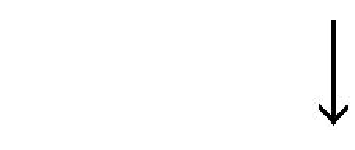
\includegraphics{down_arrow.pdf}} \end{center} \end{minipage} & \begin{minipage}[h]{1.5cm} \begin{center} \scalebox{0.35}{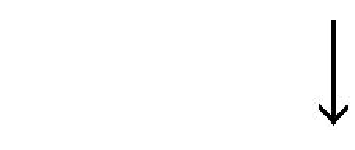
\includegraphics{down_arrow.pdf}} \end{center} \end{minipage} \\
%\vspace{0.5cm}				  
 Test statistic & $T(y)=\frac{\bar{y}_1 - \bar{y}_2}{s\sqrt{\frac{1}{n_1} + \frac{1}{n_2}}}$ & $T(y)=$ \begin{minipage}[h]{1cm} \begin{center} \scalebox{0.2}{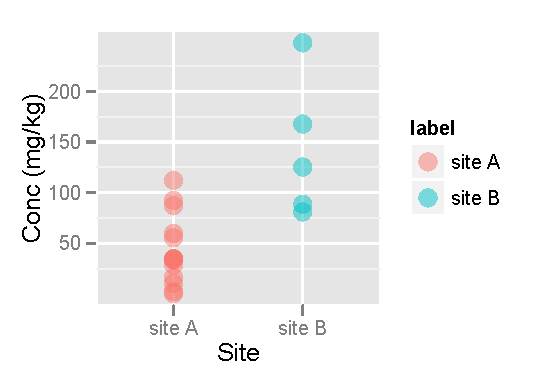
\includegraphics{data-dot.pdf}} \end{center} \end{minipage} \\
				 
 & \begin{minipage}[h]{1.5cm} \begin{center} \scalebox{0.35}{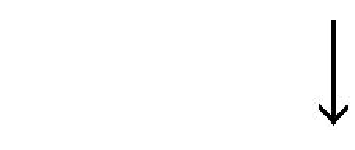
\includegraphics{down_arrow.pdf}} \end{center} \end{minipage} & \begin{minipage}[h]{1.5cm} \begin{center} \scalebox{0.35}{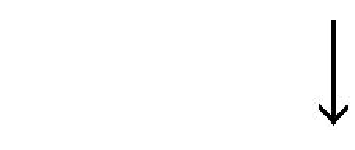
\includegraphics{down_arrow.pdf}} \end{center} \end{minipage} \\
				 
 Null Distribution & $f_{T(y)}(t); $\begin{minipage}[h]{1.5cm} \begin{center} \scalebox{0.2}{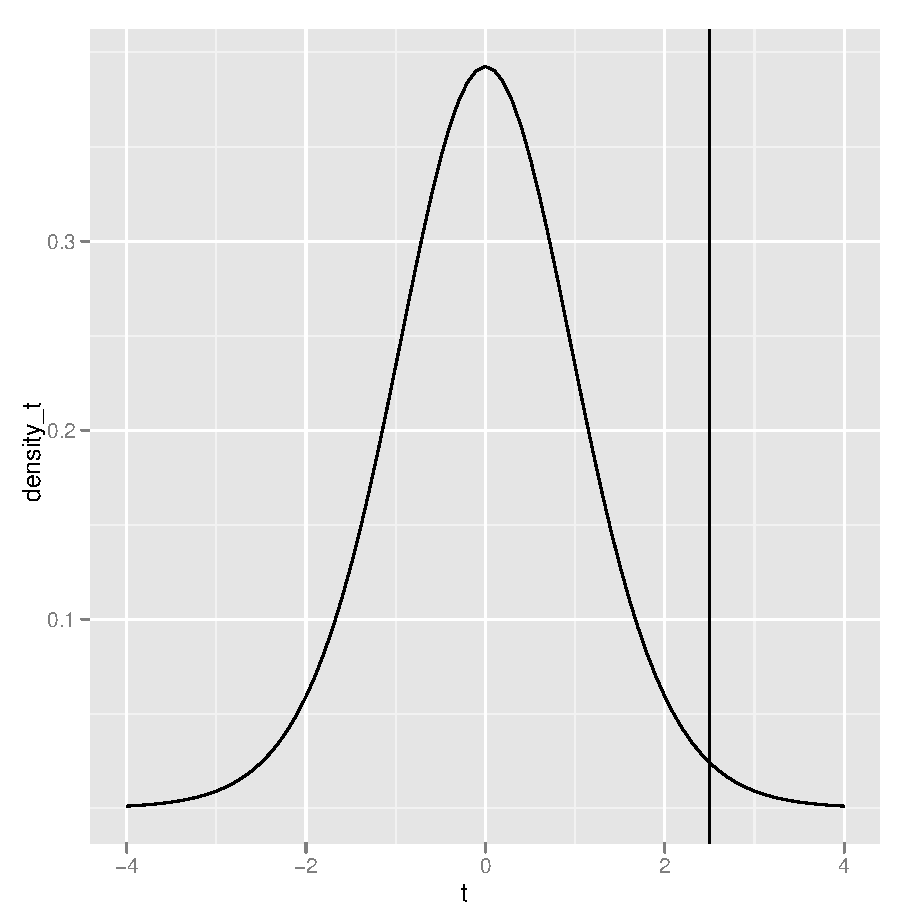
\includegraphics{stat_mathematical_test.pdf}} \end{center} \end{minipage} & $f_{T(y)}(t); $ \begin{minipage}[h]{1.5cm} \begin{center} \scalebox{0.29}{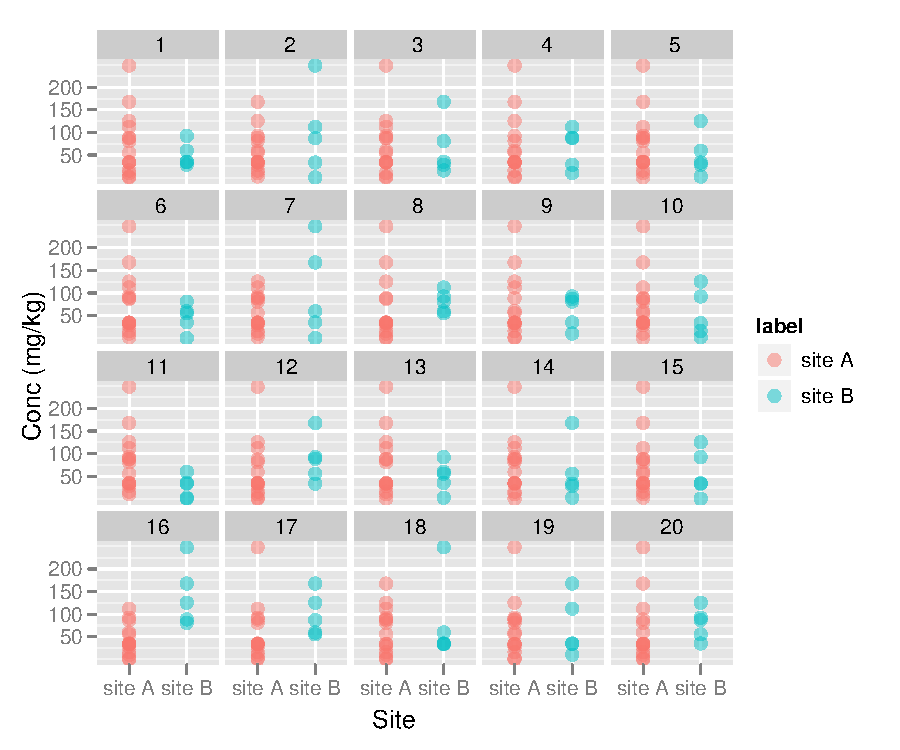
\includegraphics{lineup-dot.pdf}} \end{center} \end{minipage} \\
 & \begin{minipage}[h]{1.5cm} \begin{center} \scalebox{0.35}{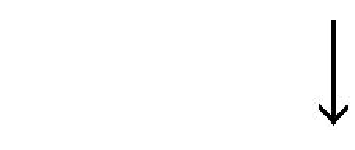
\includegraphics{down_arrow.pdf}} \end{center} \end{minipage} & \begin{minipage}[h]{1.5cm} \begin{center} \scalebox{0.35}{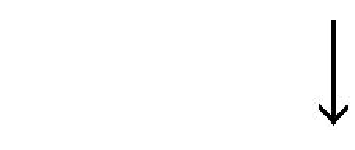
\includegraphics{down_arrow.pdf}} \end{center} \end{minipage} \\
 Reject $H_0$ if & observed $T$ is extreme & observed plot is identifiable \\
\hline 
\end{tabular}
\label{tbl:compare}
\end{table*}	

%\begin{table*}[hbtp]
%\caption{Comparison of visual inference with existing inference technique}
%\centering 
%\begin{tabular}{llll} 
%\hline
%  & Mathematical Inference &  Visual Inference \\ %[0.5ex] % inserts table %heading 
%\hline
%  Hypothesis & $H_0: \beta=0$ vs $H_a: \beta \ne 0$& $H_0: \beta=0$ vs $H_a: \beta \ne 0$\\
%%  \vspace{0.5cm}	
% & \begin{minipage}[h]{1.5cm} \begin{center} \scalebox{0.25}{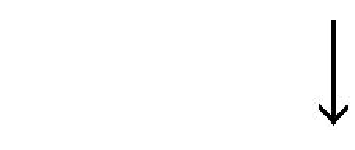
\includegraphics{down_arrow.pdf}} \end{center} \end{minipage} & \begin{minipage}[h]{1.5cm} \begin{center} \scalebox{0.25}{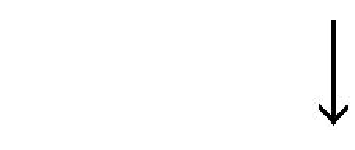
\includegraphics{down_arrow.pdf}} \end{center} \end{minipage} \\
%%\vspace{0.5cm}				  
% Test statistic & $T(y)=\frac{\hat{\beta}}{se(\hat{\beta})}$ & $T(y)=$ \begin{minipage}[h]{1cm} \begin{center} \scalebox{0.12}{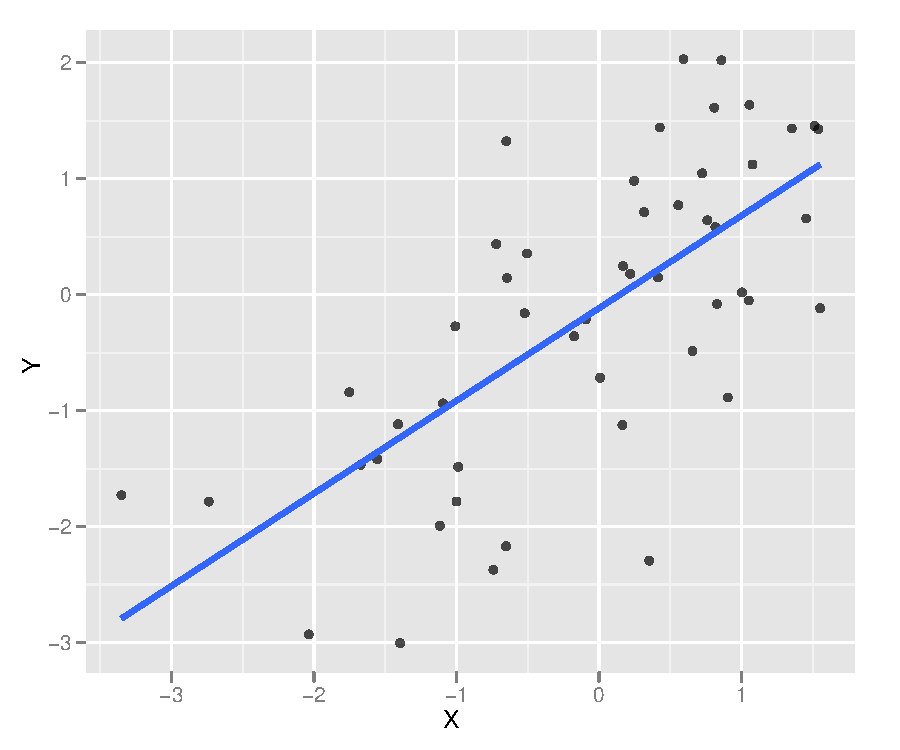
\includegraphics{test-plot.pdf}} \end{center} \end{minipage} \\
%				 
% & \begin{minipage}[h]{1.5cm} \begin{center} \scalebox{0.25}{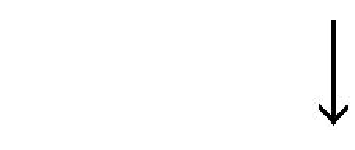
\includegraphics{down_arrow.pdf}} \end{center} \end{minipage} & \begin{minipage}[h]{1.5cm} \begin{center} \scalebox{0.25}{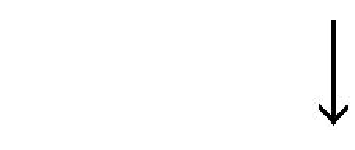
\includegraphics{down_arrow.pdf}} \end{center} \end{minipage} \\
%				 
% Null Distribution & $f_{T(y)}(t); $\begin{minipage}[h]{1.5cm} \begin{center} \scalebox{0.12}{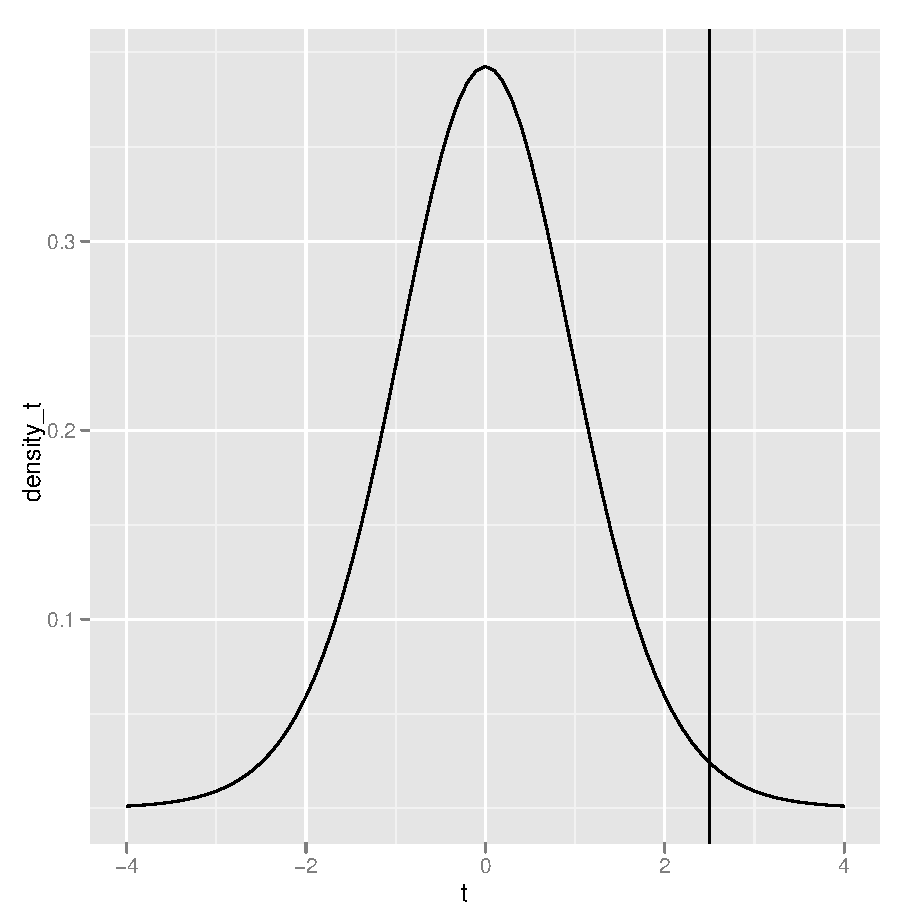
\includegraphics{stat_mathematical_test.pdf}} \end{center} \end{minipage} & $f_{T(y)}(t); $ \begin{minipage}[h]{1.5cm} \begin{center} \scalebox{0.19}{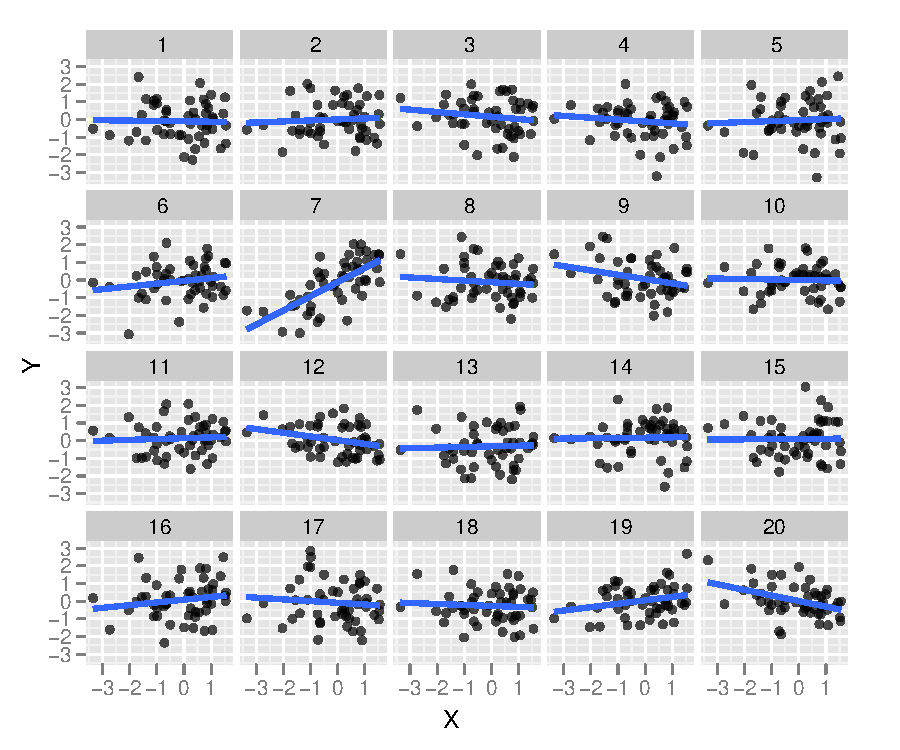
\includegraphics{stat-lineup.pdf}} \end{center} \end{minipage} \\
% & \begin{minipage}[h]{1.5cm} \begin{center} \scalebox{0.25}{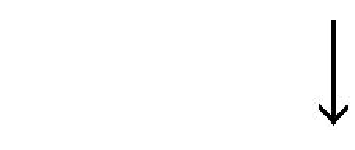
\includegraphics{down_arrow.pdf}} \end{center} \end{minipage} & \begin{minipage}[h]{1.5cm} \begin{center} \scalebox{0.25}{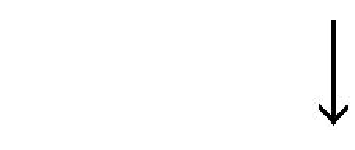
\includegraphics{down_arrow.pdf}} \end{center} \end{minipage} \\
% Reject $H_0$ if & observed $T$ is extreme & observed plot is identifiable \\
%\hline 
%\end{tabular}
%\label{tbl:compare}
%\end{table*}	


%In their paper \citet{buja:2009} presented some of the issues related to visual inference. For example the wording of the instruction for viewers while evaluating lineup plots, information related to the viewers responses, effect of colors or gaps in the plot on the responses. These issues need to be examined before more general implementation of visual inference. In my thesis work I intend to address these issues elaborately.

%\subsection{Evaluation of the Lineup Plots} Single or multiple observer can evaluate a lineup plot. If a individual observer evaluates a lineup of $m$ plots, the p-value is reported as $\le \frac1m$ when the null hypothesis is rejected and $\ge 1-\frac1m$ when the null hypothesis could not be rejected. For for a pool of $K$ observers we have $$ U \sim Binom(K,\frac1m)$$ where $U$ is the number of successful evaluations. Thus we have the p-value as $$Pr(U \ge u)= \sum_{k \ge u}^K {{K \choose k} (\frac1m)^k(1-\frac1m)^{(K-k)}}$$ where $u$ be the observed number of successful evaluations. Due to the discrete nature of binomial distribution this p-value is conservative.
%
%The type-I error probability is fixed to be $\frac1m$ as per the design of the lineup plot.

\section{Scope of my Research}

The main goal of my research is to analyze the performance of lineup protocol in various situations in finding any pattern in the data if it is actually present. My research also looks into other details and develops certain concepts in the lineup protocol. These are described below: \\

Chapter \ref{ch:largepsmalln} is an application of the lineup protocol in a large $p$, small $n$ framework. In this chapter we examine the reliability of projection pursuit methods. This chapter also provides a check on whether the separation among the groups is real or caused solely by the large number of dimensions. There are various cases when we observe separated clusters when we plot 2 dimensional projections of a $p$ dimensional data when $p$ is large compared to $n$. But the important question `Is the separation real?' We tried to answer this question in this chapter. \\

Chapter \ref{ch:waldo} takes a closer look at the null plots in a lineup. This chapter develops techniques to measure the quality of a lineup. This chapter also finds a distance measure which is the closest to the visual distance. In a lineup we compare the plot of the real data to the null plots. But since there are only a finite number of null plots we may obtain a ``bad" sample of plots. So we need to be aware of the properties of the null plots. \\

Chapter \ref{ch:teaching} develops teaching materials to improve statistical thinking among undergraduate students and among people who are familiar with statistical methods. \\ 

Chapter \ref{ch:application} would most likely use the lineup protocol to make inference in a large $n$ setting. The goal is to examine how the visual inference procedure works in a real life situation. This chapter also looks at the ``sufficient'' statistic. \\

Finally, chapter \ref{ch:conclusion} displays my completed tasks so far as well as the plans and timelines of my work for the next year. 

%\section{Validation of the Protocols}
%
%\citet{buja:2009} suggested evaluating the performance of the protocols using \cite{turk} Mechanical Turk web site. The goal is to estimate the family-wise Type I error rates for each data situation. This web site also allows us to keep record of time taken to complete a task, the reason why the individuals pick in a lineup, together with a confidence rating. Turk worker do not necessarily make-up of a representative population sample. Thus to make a correction of this selection bias we can collect some demographic information such as age, gender, education level or location of the worker. The Mechanical Turk has also been used to collect data for the Fleshmap project by \cite{viegas:2008}.
%
%We have done couple of turk studies and some results are displayed in chapter \ref{ch:regression}. More results are to be presented in chapter \ref{ch:turk} and \ref{ch:turk_analysis}.
%
%\section{Background}Statistical graph or plot of data has its presence way before the development of the classical inference procedures. The first recorded instance of statistical graphics based on the data was known to be in the year 1644 (variations in determination of longitude between Toledo and Rome as illustrated by \cite{friendly:2001}). The development of fundamental classical inferential procedures took around two hundred years from Bernoulli through Fisher (1713 to 1935 as per \cite{hald:2004}). 
%
%I intend to write down a little history of the statistical graphics in this section. The goal is to identify why the graphics were not used as a tool for statistical inference even though we see its presence way before the development of classical inference techniques. One factor could be the absence of modern computing facilities. But to what extent does the lack of computing facility prevent statistical graphics from being used as the tool for statistical inference?
%
%
%\section{Explanation of chapters and scope} I described some materials that I intend to include in chapter \ref{ch:introduction}. While one of our goals is to analyze the performance of the lineup protocol in finding the pattern of the data when it is actually present we have specific focuses in the different chapters. These are described below;
%
%Chapter \ref{ch:regression} develops the visual inference procedure for a simple linear regression setting with normally distributed error structure. The purpose is to show how the visual inference technique perform in the very fundamental inferential procedure. This chapter also provides the various methods of obtaining power of the proposed visual test. The results obtained from the human subject experiment is stunning and the paper based on these findings won the ASA student paper competition 2011. 
%
%Chapter \ref{ch:turk} describes the procedure of designing an Amazon Mechanical Turk experiment to evaluate the performance of visual inference technique. This explains the detailed factors to be considered while running the experiment. 
%
%Chapter \ref{ch:turk_analysis} is designed to present analysis of the data obtained from various turk experiments. The focus is to identify whether demographical factors are influential in visual evaluation of plots. The time taken for each evaluation may depend on the difficulty level of the plot. This will allow us to come up with some measure for the difficulty level of each lineup plot. 
%
%Chapter \ref{ch:application} focuses on the real data study. The goal is to examine how the visual inferential procedure perform in the case of real data. We intend to study the performance of line up protocols with the real data and compare them with what we obtained from simulated data.
%
%Finally chapter \ref{ch:conclusion} displays my completed tasks so far as well as the plans and timelines of my work for the next year. Some of the future directions of research are also described even though they may not be under the scope of this dissertation work. 
 
